\documentclass[12pt, letterpaper, preprint]{aastex}
%\usepackage{bm, graphicx, subfigure, amsmath, morefloats}
\bibliographystyle{apj}
\usepackage{float, bm, graphicx, subfigure, amsmath, morefloats}
\usepackage{color}
%\usepackage{caption}
%\usepackage{subcaption}
\usepackage[caption=false]{subfig}
\usepackage{tabularx}

% naming macros
\newcommand{\tc}{\textsl{The~Cannon}} 
\newcommand{\cannon}{\textsl{Cannon}} 
\newcommand{\apogee}{APOGEE}
%\newcommand{\apogee}{\textsl{APOGEE}} 
\newcommand{\aspcap}{ASPCAP}
%\newcommand{\aspcap}{\textsl{ASPCAP}}
\newcommand{\lamost}{LAMOST}
%\newcommand{\lamost}{\textsl{LAMOST}}
\newcommand{\apokasc}{APOKASC}
\newcommand{\segue}{SEGUE}
%\newcommand{\segue}{\textsl{SEGUE}}
\newcommand{\rave}{RAVE}
%\newcommand{\rave}{\textsl{RAVE}}
\newcommand{\galah}{GALAH}
%\newcommand{\galah}{\textsl{GALAH}}
\newcommand{\gaiaeso}{Gaia-ESO}
\newcommand{\gaia}{Gaia}
\newcommand{\kepler}{\textsl{Kepler}}
\newcommand{\ulyss}{\textsl{ULySS}}

% math and symbol macros
\newcommand{\set}[1]{\bm{#1}}
\newcommand{\teff}{\mbox{$\rm T_{eff}$}}
\newcommand{\feh}{\mbox{$\rm [Fe/H]$}}
\newcommand{\mh}{\mbox{$\rm [Fe/H]$}}
\newcommand{\alphafe}{\mbox{$\rm [\alpha/M]$}}
\newcommand{\alpham}{\mbox{$\rm [\alpha/M]$}}
\newcommand{\logg}{\mbox{$\rm \log g$}}
\newcommand{\ak}{\mbox{$\rm A_k$}}
\newcommand{\av}{\mbox{$\rm A_v$}}
\newcommand{\cm}{\mbox{$\rm [C/M]$}}
\newcommand{\nm}{\mbox{$\rm [N/M]$}}
\newcommand{\starlabel}{\ell}
\newcommand{\starlabelvec}{\set{\starlabel}}
\newcommand{\given}{\,|\,}
\newcommand{\angstrom}{\mbox{\AA}}

\newcommand{\ntrobj}{9952}
\newcommand{\nallobj}{454,180}
\newcommand{\ntestobj}{444,228}
\newcommand{\snr}{S/N}
\newcommand{\afebias}{-0.00247}
\newcommand{\afescat}{0.0391}
\newcommand{\tefferr}{4.4 K}
\newcommand{\nbssamples}{20}
\newcommand{\loggerr}{0.012 dex}
\newcommand{\feherr}{0.0060 dex}
\newcommand{\afeerr}{0.0042 dex}

\newcommand{\todo}[1]{{[\bf $1$]}}
\newcommand{\Comment}[2]{ [{\color{red}\sc #1 :} {{\color{cyan} \it #2}}]}

\begin{document}

\title{Label Transfer using \tc: \\
Precise Stellar Parameters for 450,000 \lamost\ Giants }
\author{Anna Y. Q. ~Ho\altaffilmark{1,2},
Melissa~K.~Ness\altaffilmark{2},
David~W.~Hogg\altaffilmark{2,3,4,5}, 
Hans-Walter~Rix\altaffilmark{2},
Chao~Liu\altaffilmark{6},
Fan~Yang\altaffilmark{6},
Yong~Zhang\altaffilmark{7},
Yonghui~Hou\altaffilmark{7},
Yuefei~Wang\altaffilmark{7}
}
\altaffiltext{1}{Cahill Center for Astrophysics, 
California Institute of Technology, MC 249-17, 
1200 E California Blvd, Pasadena, CA, 91125, USA}
\altaffiltext{2}{Max-Planck-Institut f\"ur Astronomie, 
K\"onigstuhl 17, D-69117 Heidelberg, Germany}
\altaffiltext{3}{Simons Center for Data Analysis, 
160 Fifth Avenue, 7th floor, New York, NY 10010, USA}
\altaffiltext{4}{Center for Cosmology and Particle Physics, Department of Phyics, New York University, 4 Washington Pl., 
room 424, New York, NY, 10003, USA}
\altaffiltext{5}{Center for Data Science, New York University, 
726 Broadway, 7th floor, New York, NY 10003, USA}
\altaffiltext{6}{Key Laboratory of Optical Astronomy, National Astronomical Observatories, Chinese Academy of Sciences, Datun Road 20A, Beijing 100012, China}
\altaffiltext{7}{Nanjing Institute of Astronomical Optics \& Technology, National Astronomical Observatories, Chinese Academy of Sciences, Nanjing 210042, China}

\email{ah@astro.caltech.edu}

\begin{abstract}

To capitalize on a diverse set of large spectroscopic stellar surveys,
it is essential to develop techniques for precise and accurate survey cross-calibration.
Here, we demonstrate that this can be achieved by a data-driven approach to spectral modeling: we use \tc\ \citep{Ness2015} to
cross-calibrate \apogee\ and \lamost, 
two large-scale surveys
that currently yield inconsistent results
due to differing experimental setups and data
analysis methodologies.
\tc\ constructs a predictive model for \lamost\ spectra 
using a reference set of \ntrobj\ stars observed in common between the two surveys, taking five labels as ground truth from \apogee\ DR12:
\teff, \logg, \feh, \alpham, and K-band extinction \ak.
The model is then used to infer 
\teff, \logg, \feh, and \alpham\
for \nallobj\ giant stars in \lamost\ DR2,
thus tying low-resolution (R\,$\sim$\,1800) \lamost\ spectra to the
\apogee\ (R\,$\sim$\,22,500) label scale.
Despite being derived directly from \lamost\ spectra,
which have lower spectral resolution and very different
wavelength coverage,
these new Cannon labels have an accuracy and precision comparable to the stated \apogee\ DR12 values and uncertainties,
essentially eliminating the systematic label inconsistencies resulting from the individual survey pipelines.
By transferring \alpham\ labels from \apogee ,  \tc\ produces the first \alpham\ values measured from \lamost\ spectra, and the largest catalog of \alpham\ for giant stars to date.
This demonstrates that \tc\ can
successfully bring different surveys onto the same label scale,
and effectively transfer label systems from a high-resolution
survey to low-resolution spectra.

\end{abstract}

\keywords{
catalogs
---
methods: data analysis
---
methods: statistical
---
stars: abundances
---
stars: fundamental parameters
---
techniques: spectroscopic
}

\section{Survey Cross-Calibration With \tc }

A diverse suite of large-scale spectroscopic stellar surveys
(e.g. 
\apogee\ \citep{Majewski2015},
\gaiaeso\ \citep{Gilmore2012},
\galah\ \citep{DeSilva2015},
\lamost\ \citep{Zhao2012},
\rave\ \citep{Kordopatis2013}, and
\segue\ \citep{Yanny2009})
have been measuring spectra for hundreds of thousands of stars in the Milky Way.
They target different types of stars, in different parts of the sky, and at different wavelengths.
For example, \apogee\ observes in the near-infrared (near-IR)
and targets predominantly giants in the dust-obscured mid-plane of the Galaxy,
whereas \galah\ observes in the optical and targets
predominantly nearby main sequence stars. 
In addition, they observe at different resolutions and
employ different data analysis methodologies for using
spectra to derive a set of labels characterizing the star,
e.g. \teff , \logg , \alpham, and [X/H].

These surveys are complementary in their spatial coverage and scientific motivation,
and there is enormous scientific promise in combining their results.
However, diversity is also the reason why surveys cannot be rigorously stitched together at present:
different pipelines measure substantially different labels for the same stars (e.g. \citet{Smiljanic2014}). 
For example, \citet{Chen2015} compared the three stellar parameters \teff, \logg, and \feh\ between \apogee\ and \lamost, two of the most ambitious ongoing surveys, and found consistency in the photometrically-calibrated \teff\
but systematic biases in \logg\ and \feh, as 
Figure \ref{fig:apogee-lamost} shows for \ntrobj\ objects 
observed and analyzed by both surveys. 

Although such systematic label offsets may not be surprising for two surveys with disjoint wavelength coverage and very different spectral resolutions (see Section \ref{sec:data}), labels are ultimately characteristics of stars and not of observations, and must therefore be unbiased and consistent between surveys to within the stated error bars.
To that end, better techniques must be developed for bringing different surveys onto the same label scale. 

\begin{figure}[!p]
\centering
\includegraphics[scale=0.5]{f1.eps}
\caption{Systematic offsets in the labels
\teff, \logg, and \feh\
derived by the \lamost\ and \apogee\ pipelines, for \ntrobj\ stars that
have been observed and analyzed by both surveys.
There are strong biases in \logg\ and \feh.
The panel rows show subsets of different \lamost\ \snr, calculated for each spectrum by taking
the median of the flux-uncertainty ratio across all pixels.
}
\label{fig:apogee-lamost}
\end{figure}

We approach this cross-calibration problem using \tc\ \citep{Ness2015}, a new data-driven method for measuring stellar labels from stellar spectra in the context of large spectroscopic surveys. 
\citet{Ness2015} describe the method and its application to \apogee\ DR10 spectra in detail, and \citet{NessAges} use \tc\ and the \apokasc\ sample to determine masses and ages directly from \apogee\ spectra. 
Here, we recapitulate the fundamental assumptions and steps
of \tc\ in the context of survey cross-calibration, and
describe the procedure more concretely in sections 
\ref{sec:training} and \ref{sec:test}. 

Presume that our goal is to cross-calibrate Survey A and Survey B,
two spectral surveys that are not (yet) on the same label scale (in other words, the Survey A and Survey B pipelines measure inconsistent labels for objects
observed in common, as in Figure \ref{fig:apogee-lamost}.) 
Presume further that we trust Survey A's labels more than Survey B's
(e.g. because Survey A has higher spectral resolution and higher \snr) and therefore aim to cross-calibrate by bringing Survey B onto Survey A's label scale.

\tc\ relies on a few key assumptions: 
that stars with identical labels have very similar spectra, and that spectra vary smoothly with label changes.  
In other words, the continuum-normalized flux at each pixel in a spectrum is a smooth function of the labels that describe the object. 
The function that takes the labels and predicts the 
flux at each wavelength of the spectrum is called the ``spectral model"; 
fitting for the coefficients of the spectral model is the goal of the first step, 
the ``training'' step.

In the training step, \tc\ uses the objects with spectra from Survey B and labels from Survey A
as ``reference objects" to fit for the spectral model coefficients at each pixel of the spectrum independently.
The spectral model characterizes the flux at each pixel of a Survey B 
spectrum as a function of corresponding Survey A labels, and
predicts what the spectrum of an object observed in Survey B
would look like given a set of labels from Survey A. 

In the second step, the ``test" step, this model is used to derive 
likely labels for any (similar) object given its spectrum from Survey B,
including those not observed by Survey A. 
Note that if the Survey A pipeline has measured a dozen labels precisely and the 
Survey B pipeline has only measured three, we can in principle use
our model to infer extra, previously unknown labels from Survey B spectra; we dub this process of transferring knowledge of labels from one survey to another ``label transfer." 
Note also that in this approach, Survey A enters only through its labels, not the data (spectra, light curves, or otherwise) from which these labels were derived, and Survey B enters only through its spectra. 

In this work, we take \apogee\ to be Survey A and \lamost\ to be Survey B. 
We select \apogee\ as the source of the trusted stellar
labels because it is the higher-resolution survey ($R\approx22,500$ versus $R\approx1,800$ for \lamost).
We use five post-calibrated labels from \apogee\ DR12: \teff, \logg, \feh, \alpham, and K-band extinction \ak. While \ak\ is not strictly an intrinsic property of the stars, it is a ``label'',
in the sense that it is an immutable property of the stellar spectrum when observed from our location in the Galaxy.
We decided to include extinction in constructing the model because 
the objects in the reference set (in the Galactic mid-plane) 
include visual extinctions up to \av\,$\approx$\,3.5 (\ak\,$\approx$\,0.4).
This impacts some of the optical spectra in the training step and in the test step,
not only by reddening, but also by dust and gas absorption features. 

Note that what we call \feh\ in this work is stored under the header \texttt{PARAM\_M\_H} in DR12. 
We use this value so that all four labels have gone through the same post-calibration procedure, but refer to it as \feh\ rather than [M/H] because it has been calibrated to the \feh\ of star clusters \citep{Meszaros2013}, and in order to be consistent with the terminology
from \lamost.

The 11,057 objects measured in common between \apogee\ and \lamost\ constitute the possible reference set for the training step;
in practice, we use \ntrobj\ of these objects to fit for 
the spectral model, then apply this model 
to infer both new labels for the reference set,
as well as labels for the remaining 
\ntestobj\ \lamost\ giants in DR2 \emph{not} observed by \apogee.
By construction, these labels are tied to the \apogee\ scale.

This work and \citet{Ness2015} share the same general procedure.
The fact that it performs well for spectra at very different wavelength regimes and resolutions illustrates the general applicability of this procedure to large uniform sets of stellar spectra, given a suitable reference set.
The methodology is described in detail in \citet{Ness2015} and the
procedure here is simply an implementation;
the primary distinguishing feature
in how the \lamost\ spectra were prepared for \tc,
and we describe that process in Section \ref{sec:normalization}.

\section{Data: \lamost\ Spectra and \apogee\ Labels}\label{sec:data}

The Large sky Area Multi-Object Spectroscopic Telescope (\lamost) 
is a low-resolution ($R\approx1,800$) optical ($3650-9000\,\angstrom$) spectroscopic survey.
As of the second data release (DR2; \citet{Luo2015}), \lamost\ has 
obtained spectra for over 4.1 million objects and 
measured three stellar labels (\teff, \logg, \feh) for
 $\sim\,$2.2 million stars. 
Although the survey does not select for
a particular stellar type, many of the stars
are red giants; the population of K giants
numbers 300,000 in DR1 and 500,000 in DR2
\citep{Liu2014}. 
Moreover, \textgreater\,100,000 red clump candidates have been identified in the DR2 catalog \citep{Wan2015}.
Stellar labels for the \lamost\ spectra 
are derived by
the package \ulyss\ \citep{Wu2011}, which fits each spectrum to a 
model spectrum that is a linear combination of non-linear components,
optically convolved with a line-of-sight velocity
distribution and multiplied by a polynomial function. 
Improved surface gravity values have been obtained for
the metal-rich giant stars via cross-calibration with asteroseismically-derived values from
\kepler\ \citep{Liu2015}.

\apogee\ is a high-resolution ($R\approx22,500$), high-\snr\ (\snr\ $\approx100$), H-band (15200-16900\,$\mbox{\AA}$) spectroscopic survey, part of the Sloan Digital Sky
Survey III (\citet{Majewski2015,Eisenstein2011}). 
Observations are conducted using a 300-fiber spectrograph
\citep{Wilson2010} on the 2.5\,m Sloan Telescope
\citep{Gunn2006} at the Apache Point Observatory (APO) in Sunspot, New Mexico (USA) and consist primarily of
red giants in the Milky Way bulge, disk, and halo.
The most recent data release, DR12 \citep{Alam2015, Holtzman2015},
comprises spectra for \textgreater\,100,000 red giant stars together with their basic stellar parameters and 15 chemical
abundances. 
The parameters and abundances are 
derived by the ASPCAP pipeline, which is based on chi-squared fitting of the data to 1D LTE models for seven labels: \teff, \logg, \feh, \alpham, \cm, \nm, and micro-turbulence \citep{GarciaPerez2015}. 

\subsection{Preparing \lamost\ Spectra for \tc} 
\label{sec:normalization}

To be used by \tc, any spectroscopic data set must satisfy the conditions laid out in \citet{Ness2015}. 
The spectra must share a common line-spread function, be shifted to the rest-frame and sampled onto a common wavelength grid with uniform start and end wavelengths.
The flux at each pixel of each spectrum must be accompanied
by a flux variance that takes error sources such as photon noise and poor sky subtraction into account; 
bad data (e.g. regions with skylines and telluric regions) must be
assigned inverse variances of zero or very close to zero.
Finally, the spectra do not need to be continuum normalized, but they must be normalized
in a consistent way that is independent of S/N; 
more precisely, the normalization procedure should be a linear operation on the data, so that it is unbiased as (symmetric) noise grows. 

Preparatory steps were necessary to make the raw \lamost\ spectra
satisfy these criteria.
First, the displacement from the rest-frame was
calculated for each spectrum using the redshift value provided in 
the data file header, and the spectra shifted accordingly.
(The redshift values are derived within the \lamost\ 
data pipeline, 
from their cross-correlation procedure.)
Spectra were then re-sampled onto the original grid using linear interpolation. 
After shifting, we applied lower and upper wavelength cuts
and sampled all spectra onto a common wavelength grid 
spanning 3905\,$\mbox{\AA}$ -- 9000\,$\mbox{\AA}$.
All of these operations were performed on both the flux and inverse variance
arrays. 

Each spectrum was normalized by dividing the flux at each $\lambda_0$ by $\bar{f} (\lambda_0)$, which was
derived by an error-weighted, broad Gaussian smoothing:

\begin{equation}
\bar{f}(\lambda_0) = \frac{\sum_i (f_i\,\sigma^{-2}_i\,w_i(\lambda_0))}{\sum_i (\sigma^{-2}_i\,w_i(\lambda_0))},
\end{equation}

\noindent where $f_i$ is the flux at pixel $i$, $\sigma_i$ is the uncertainty at pixel $i$, and the weight $w_i (\lambda_0)$ is drawn from a Gaussian 

\begin{equation}
w_i(\lambda_0) = e^{-\frac{(\lambda_0-\lambda_i)^2}{L^2}},
\end{equation}

\noindent $L$ was chosen to be 50\,$\mbox{\AA}$,
much broader than typical atomic lines. 

To emphasize, this ``normalization'' is in no sense
``continuum normalization,'' and is
different from the standard normalization used in
spectral analysis. Our goal in preparing the spectra in this way is to simplify the modeling procedure by removing overall flux, flux calibration, and large-scale shape changes from the spectra.

The procedure is illustrated in Figure \ref{fig:sample_spec}, 
which shows three spectra corresponding to a sample reference object: 
its \apogee\ spectrum, its \lamost\ spectrum overlaid with its Gaussian-smoothed  ``continuum," and final ``normalized" \lamost\ spectrum. 

\begin{figure}[!p]
\centering
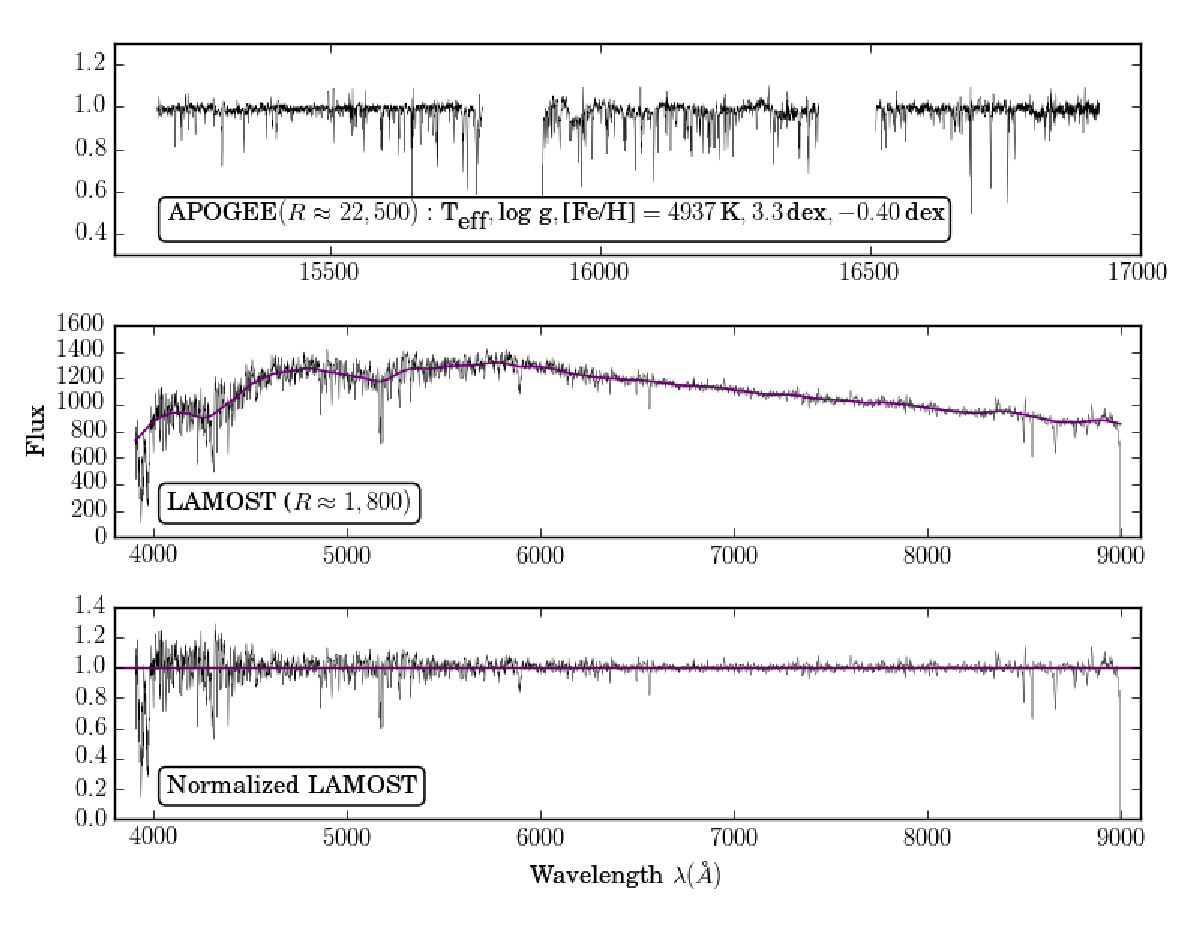
\includegraphics[scale=0.85]{f2.eps}
\caption{Spectra of a sample reference object (2MASS ID 2M07101078+2931576).
The top panel shows the normalized \apogee\ spectrum (with its basic stellar labels) and the middle panel shows
the raw \lamost\ spectrum overlaid with the Gaussian-smoothed version of itself. 
The bottom panel shows the resulting ``normalized" spectrum, determined by
dividing the black line by the purple line in the middle panel. \tc\ operates on the normalized
spectrum in the bottom panel, although note that this ``normalization'' is different from the standard normalization used in spectral analysis. 
\apogee\ and \lamost\ spectra are qualitatively 
very different, in wavelength coverage and resolution.}
\label{fig:sample_spec}
\end{figure}

\section{\tc\ Training Step: \\ Modeling \lamost\ Spectra as a Function of \apogee\ Labels}
\label{sec:training}

Our reference set comprises \ntrobj\ of the 11,057 objects measured in common between \lamost\ DR2 and \apogee\ DR12. 
We eliminate stars with
unreliable \teff, \logg, \feh, \alpham, or \ak\, as described in \citet{Holtzman2015}.
Initially, we excise objects with 3500\,\textless\,\teff\,\textless\,6000, 
with \alpham\,\textless\,0.1\,dex, 
or with \texttt{ASPCAPFLAG} set.
We then train the model on the remaining objects, apply this model
to the reference set (cross-calibration) and discard objects 
whose difference from the reference (\apogee) value
in any particular label is greater than four times the scatter in that label.
This leaves \ntrobj\ objects.

The distribution of these \ntrobj\ reference objects in (\lamost\ \teff, \lamost\ \logg) label space is shown in 
Figure \ref{fig:reference-set-label-space}. The black points in the background are the full
\lamost\ DR2 sample, with their values from the \lamost\ pipeline. 
The overlaid colored points are the reference objects; in the left panel, they are shown with their
\lamost\ pipeline values, and in the right panel, they are shown with their \apogee\ pipeline values.
It is only the \apogee\ labels, shown as colored dots in the right panel,
that are used in the training step. 

\begin{figure}[H]
\centering
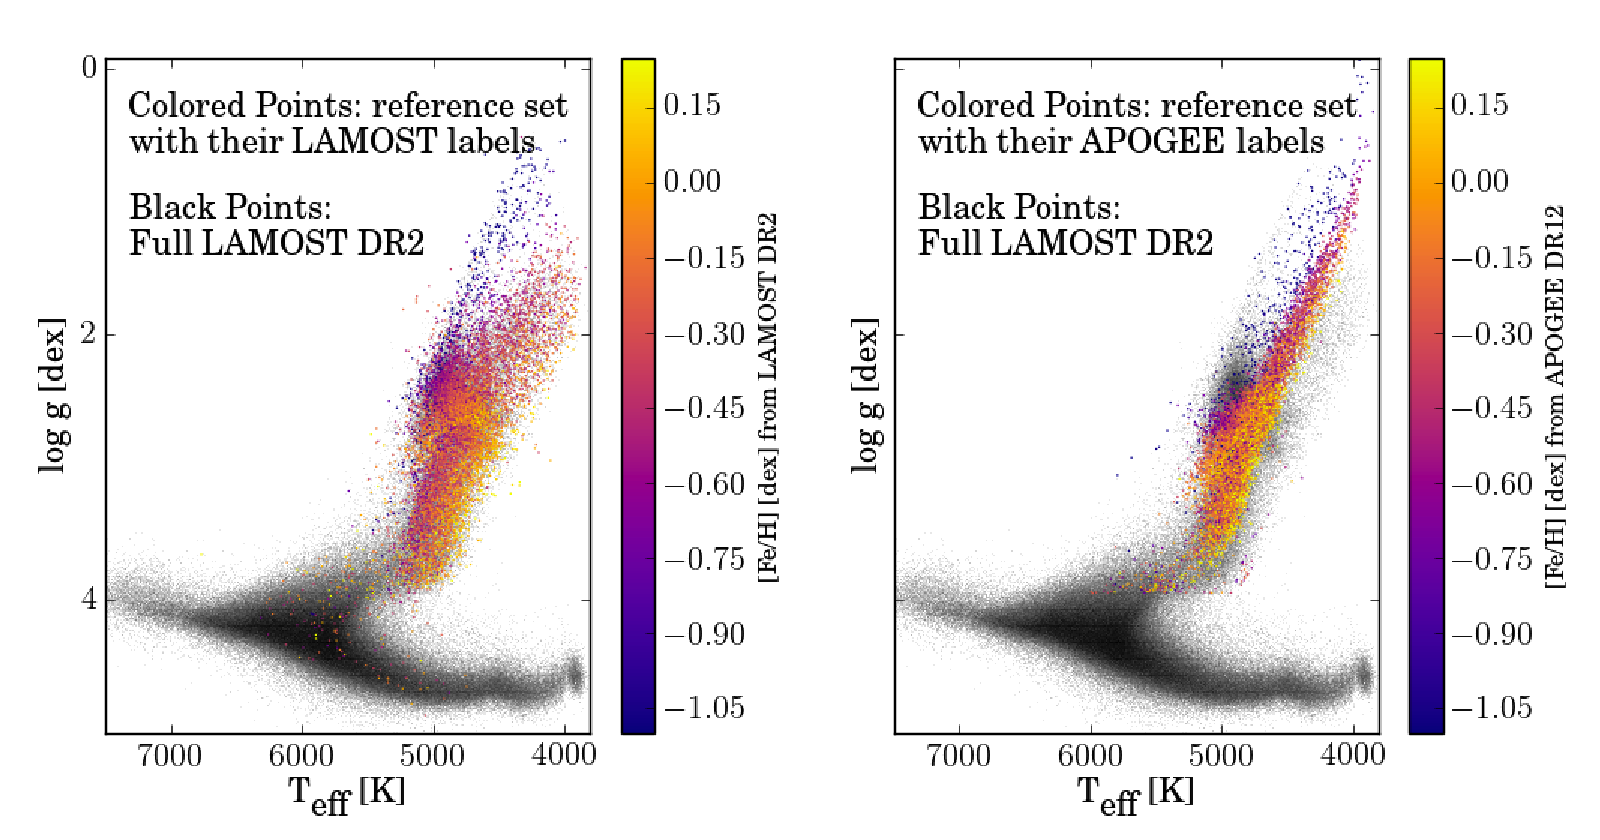
\includegraphics[scale=0.6]{f3.eps}
\caption{
LAMOST DR2 (black points), overlaid with the reference set of \ntrobj\ objects (colored points) used to train the spectral model.
These colored points are objects that have been observed by both \lamost\ and \apogee;
in the left panel, they are shown with their
\lamost\ pipeline values, and in the right panel, they are shown with their \apogee\ pipeline values.
It is the values in the right panel that are used to train the spectral model.}
\label{fig:reference-set-label-space}
\end{figure}

\tc\ uses the reference objects to fit for a spectral model that characterizes the flux
in each pixel of the (normalized) spectrum as a function $g$ of the labels of the star. 
In general, the flux $f_{n\lambda}^B$ for object $n$ at wavelength $\lambda$ in Survey B can be written as

\begin{eqnarray}
f_{n\lambda}^B &=&
g(\starlabelvec^A_n |  \set{\theta}_\lambda) + \mbox{noise}
\label{eq:specmodel}\quad 
\end{eqnarray}

\noindent where $\set{\theta}_\lambda$ is the set of 
spectral model coefficients at each wavelength $\lambda$ of the Survey B spectrum and
$\starlabelvec^A_n$ is some (possibly complicated) function of the full set of labels (from Survey A). 
The noise model is $\mbox{noise} = [s_\lambda^2+ \sigma_{n\lambda}^2]\,\xi_{n\lambda}$,
where each $\xi_{n\lambda}$ is a Gaussian random number with zero mean and unit variance. 
The noise is thus a root-mean-square (rms) combination of inherent uncertainty in the spectrum
from e.g. instrument effects and finite photon counts ($\sigma_{n\lambda}$) and 
intrinsic scatter in the model at each wavelength ($s_\lambda$). 
Handling uncertainties by fitting for a noise model
independently at each pixel is a key feature of \tc\ and 
distinguishes it from traditional machine learning methods. 

Following \citet{Ness2015} we presume that the model $g$ can be written 
 as a linear function of $\starlabelvec_n$: 

\begin{eqnarray}
f_{n\lambda}^B &=&
\set{\theta}_\lambda^T \cdot \starlabelvec^A_n + \mbox{noise}
\label{eq:linearmodel}\quad
\end{eqnarray}

\noindent corresponding to the single-pixel log likelihood function

\begin{eqnarray}
\ln p(f_{n\lambda}^B\given\set{\theta}^T_\lambda, \starlabelvec^A_n, s_\lambda^2) &=&
 -\frac{1}{2}\,\frac{[f_{n\lambda}^B - \set{\theta}^T_\lambda \cdot \starlabelvec^A_n]^2}{s_\lambda^2 + \sigma_{n\lambda}^2}
 -\frac{1}{2}\,\ln(s_\lambda^2 + \sigma_{n\lambda}^2)
\label{eq:like}\quad.
\end{eqnarray}

\noindent For this work, once more as in \citet{Ness2015}, 
we use a quadratic model such that $\starlabelvec_n$ is  

\begin{equation}
\begin{aligned}
\starlabelvec^A_n \equiv 
& \Bigl [1, \teff, \logg, \feh, \alpham, \ak, \\
& \teff\cdot\logg, \teff\cdot\feh, \teff\cdot\alpham, \teff\cdot\ak, \logg\cdot\feh, \logg\cdot\alpham, \\
& \logg\cdot\ak, \feh\cdot\alpham, \feh\cdot\ak,
\alpham\cdot\ak, \\
& \teff^2, \logg^2, \feh^2, \alpham^2, \ak^2  \Bigr 
]_{\mathrm{Survey A}}
\label{eq:quadinthreelabels}
\end{aligned}
\end{equation}

The training step thus consists of holding the labels in the label vector $\starlabelvec^A_n$ fixed (these are the reference labels) and optimizing the log likelihood to solve for the coefficients 
$[\theta_\lambda, s_\lambda^2]$ independently at every pixel. 
For a fixed scatter value, optimization is a pure linear-algebra operation (weighted least squares). 
Currently, we optimize for the scatter by stepping through a grid of scatter values. 

Figure \ref{fig:leading-coeffs} shows the leading (linear) coefficient for each label as
a function of wavelength, as well as the scatter as a function of wavelength.
The magnitude of the leading coefficient can be thought of as the sensitivity 
of a particular pixel is to that particular label. Thus, Figure \ref{fig:leading-coeffs}
is a way to visualize which regions of the spectrum are (as determined by
\tc) important for which labels. 
We find that \teff, \logg, \feh, and
\alpham\ all have strong
sensitivity to well-known spectral features such as
Mg I, Na I D, and the Ca II triplet. 

Interestingly, we find that \ak\ has strong sensitivity not only to the Na I D doublet, but also to features that correspond
to known diffuse interstellar bands (DIBs).
The strongest of these DIBs are indicated by the
orange lines in the lower panels of
Figure \ref{fig:leading-coeffs}.
DIBs are absorption features that appear to arise from diffuse
interstellar material; see \citet{Sarre2006} and \citet{Herbig1995}
for extensive reviews. 
Over four hundred have been detected to date, mostly at optical
wavelengths, but their origin remains uncertain \citep{Hobbs2008,Herbig1993}.
DIB strength has been found to correlate well with extinction and the column density of neutral hydrogen \citep{Friedman2011}. 
In addition, some DIBs seem to have correlated strengths, which suggests a shared origin \citep{McCall2010,Friedman2011}. 
Large-scale studies of DIBs (e.g. \citet{Yuan2012}) hold promise for learning not only about their origin but also for mapping their environment; \citet{Zasowski2015}
used DIBs in \apogee\ infrared spectra to find that
DIB strength is linearly correlated with extinction and thus a powerful probe of the structure and properties of the ISM.
It is therefore perhaps not surprising that \tc\ learned to associate
\ak\ with DIB strength; features in the leading coefficients plot
include well-known DIBs, e.g. at
4428\,\angstrom, 4882\,\angstrom, 5780\,\angstrom, 
5797\,\angstrom, 6203\,\angstrom, 6283\,\angstrom,
6614\,\angstrom, and 8621\,\angstrom.
Note that the DIBs in the Cannon model are effectively
smeared across the radial velocity dispersion of the training
sample.

\begin{figure}[!p]
\centering
\includegraphics[scale=0.85]{f4.eps}
\caption{Leading (linear) coefficients and scatter from the best-fit spectral model, with prominent features labeled.
These coefficients indicate how sensitive each pixel in the spectrum is to each of the labels.
In the top four panels, note peaks at well-known spectral features such as the Mg I triplet around 5170 \angstrom\ and the Ca II triplet around 8600 \angstrom. In the fifth panel, 
note peaks at well-known diffuse interstellar bands (DIBs).
The coefficients are scaled by the approximate errors in the labels
(91.5~K in \teff, 0.11 in \logg, 0.05 in \feh\ and \alpham; \citet{Holtzman2015}). 
}
\label{fig:leading-coeffs}
\end{figure}

\section{\tc\ Test Step: \\ Deriving New Stellar Labels from \lamost\ Spectra}
\label{sec:test}

In the training step (see Section \ref{sec:training}), we
treated the labels $\starlabelvec^A_n$ as known and 
solved for the coefficients $\set{\theta}_\lambda$ of the spectral model. 
Now, in the test step, we take these spectral model coefficients
and solve for new labels $\starlabelvec^B_n$ 
(as opposed to $\starlabelvec^A_n$), based on the 
spectra $f_{n\lambda}^B$ for each test object $n$.
For a model that is quadratic in the labels, 
like ours, this consists of non-linear optimization. 
We use Python's $\texttt{curve\_fit}$ routine with seven 
starting points in label space, to assure convergence. 

Before deriving new stellar labels for \lamost\ objects, 
we feed the \ntrobj\ reference objects back into \tc\ for cross-validation.  
Figure \ref{fig:cross-validation} shows the four labels
(\teff, \logg, \feh\, and \alpham) as determined by \tc\ directly
from \lamost\ spectra,
plotted against the corresponding \apogee\ (reference) labels, determined by \aspcap\ directly from \apogee\ spectra. 
For completeness, we show the output for extinction in the 
final panel (light purple).
Note that, in this work, we consider extinction as a ``nuisance''
label: we fit for it in order to more reliably determine
the four other labels, but the question of how to use \tc\ to reliably determine extinction values from spectra is beyond the scope of this work.
The low scatter and bias in the \alpham\ panel (bottom right)
shows how well \tc\ transferred a {\sl new} label
to the \lamost\ data set.
The scatter in all four labels for the objects with high \snr\ \lamost\ spectra is comparable to the typical uncertainties from  ASPCAP:  91.5~K in \teff, 0.11 in 
\logg, and around 0.05 in both \feh\ and \alpham\  \citep{Holtzman2015}. Note that the scatter in \alpham\ derived from the \lamost\ spectra is very similar to the precision in $[\alpha /Fe]$ inferred indirectly for the Segue G-dwarfs by \citet{Bovy2012},
based on SDSS spectra at similar resolution, wavelength coverage and \snr. 

This information is represented as residuals in
Figure \ref{fig:apogee-cannon}; a direct comparison with
Figure \ref{fig:apogee-lamost} shows a significant
improvement in scatter and a dramatic reduction of systematic
differences between the labels derived from \lamost\ and \apogee\  spectra, particularly in \logg\ and \feh .
The inter-survey biases in the three labels have all but vanished,
demonstrating that we have successfully measured \apogee-scale labels 
directly from \lamost\ spectra, thus bringing the two
surveys onto the same scale.
Note also, that the scatter (at a given \snr) has 
been reduced considerably: \tc\ can also measure more precise labels 
from the low-resolution \lamost\ spectra \citep{Ness2015}. 

\begin{figure}[!p]
\centering
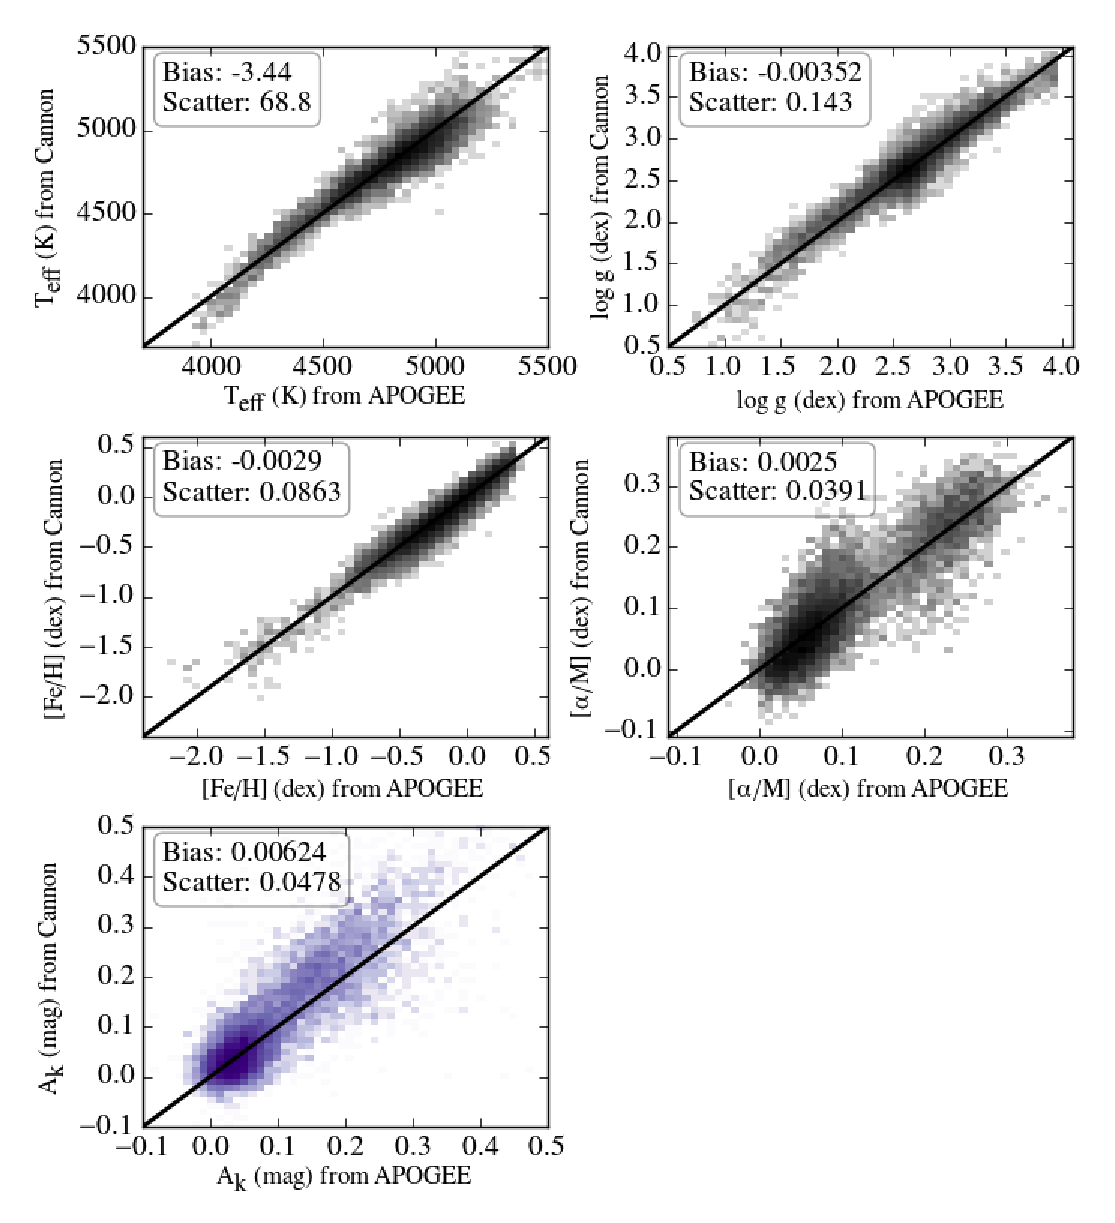
\includegraphics[scale=0.73]{f5.eps}
\caption{Cross-validation of \tc 's label transfer from \apogee\ to \lamost~: Shown are the \apogee\ labels of all reference objects compared to the labels derived from \lamost\ data by \tc\ in the test step. Strictly speaking, this is a leave-none-out test, but we have verified that training on 80\% of the reference set and testing on the remaining 20\% gives consistent results. The tight one-to-one correlations in the \teff , \logg~ and \feh\ panels simply reflect the quality of the label transfer demonstrated already in Figure \ref{fig:apogee-cannon}.
The bottom right panel shows how well \tc\ is able to transfer the {\sl new} label  \alpham~ from \apogee.
For completeness, we include extinction as a fifth panel, 
but emphasize that ours is not a reliable method for 
inferring extinction from \lamost\ spectra.
The scatter and bias values represent spectra with \snr\textgreater\,50.
}
\label{fig:cross-validation}
\end{figure}

\begin{figure}[!p]
\centering
\includegraphics[scale=0.5]{f6.eps}
\caption{Comparison between \tc\ output and \apogee\ reference labels~: Shown here are labels for the \ntrobj\ in the reference set, objects measured in common between \lamost\ and \apogee.
The systematic differences between labels determined by \tc\ from \lamost\ spectra and by \aspcap\ from \apogee\ spectra have been almost completely eliminated (see (Figure \ref{fig:apogee-lamost}).
The Cannon values also show a substantially reduced scatter with respect to the \apogee-labels, presumed to be ground-truth here.
}
\label{fig:apogee-cannon}
\end{figure}

Furthermore, \tc\ performs more precisely at low \snr\
than the \lamost\ pipeline, as seen in Figure \ref{fig:snr-test}. 
Here, for a \snr\ metric, we define ``$\sim\,\mathrm{SNR}_\mathrm{g}$.''
We quantify \snr\ in the g-band because the leading coefficients
show that decisive information comes from this regime.
Furthermore, the error bar and \snr\ should reflect the
variance of each pixel around the best-fit model; 
thus, the $\chi^2$ of a model that fits well (in this case, 
the model from \tc) should roughly equal the number of pixels in the spectrum, 3626. 
Instead, the $\chi^2$ led us to find that the errors and \snr\ in the spectra needed to be adjusted by a factor of three. 
Thus, $\sim\,\mathrm{SNR}_\mathrm{g}$ represents the \snr\ in the
g-band, multiplied by three.

\begin{figure}[!p]
\centering
\includegraphics[scale=0.7]{f7.eps}
\caption{The \snr-dependence of the scatter between
\apogee\ DR12 labels and the corresponding labels measured from
\lamost\ spectra by \tc\ (red points) and \ulyss\ (blue points).
\tc\ represents a substantial improvement from the
\lamost\ pipeline in the three labels that the 
the \apogee\ and \lamost\ pipelines measure in common.
The performance improvement is generally steeper than the
inverse of the \snr.
Note that we are using our own value for $\sim\,\mathrm{SNR}_\mathrm{g}$, which does not reflect
the reported LAMOST error bar.
}
\label{fig:snr-test}
\end{figure}

Figure \ref{fig:red-clump} provides verification that the label transfer in \teff\ and \logg\ has led to astrophysically plausible results. It compares the (\teff, \logg) distribution for all reference objects using their labels from the \apogee\ pipeline, from the \lamost\ pipeline, and from the Cannon model for the \lamost\  data. Both the morphology of the red clump and of the giant branch shows that the Cannon labels are physically much more plausible than the pipeline labels derived from the same \lamost\ data.  

\begin{figure}[H]
\centering
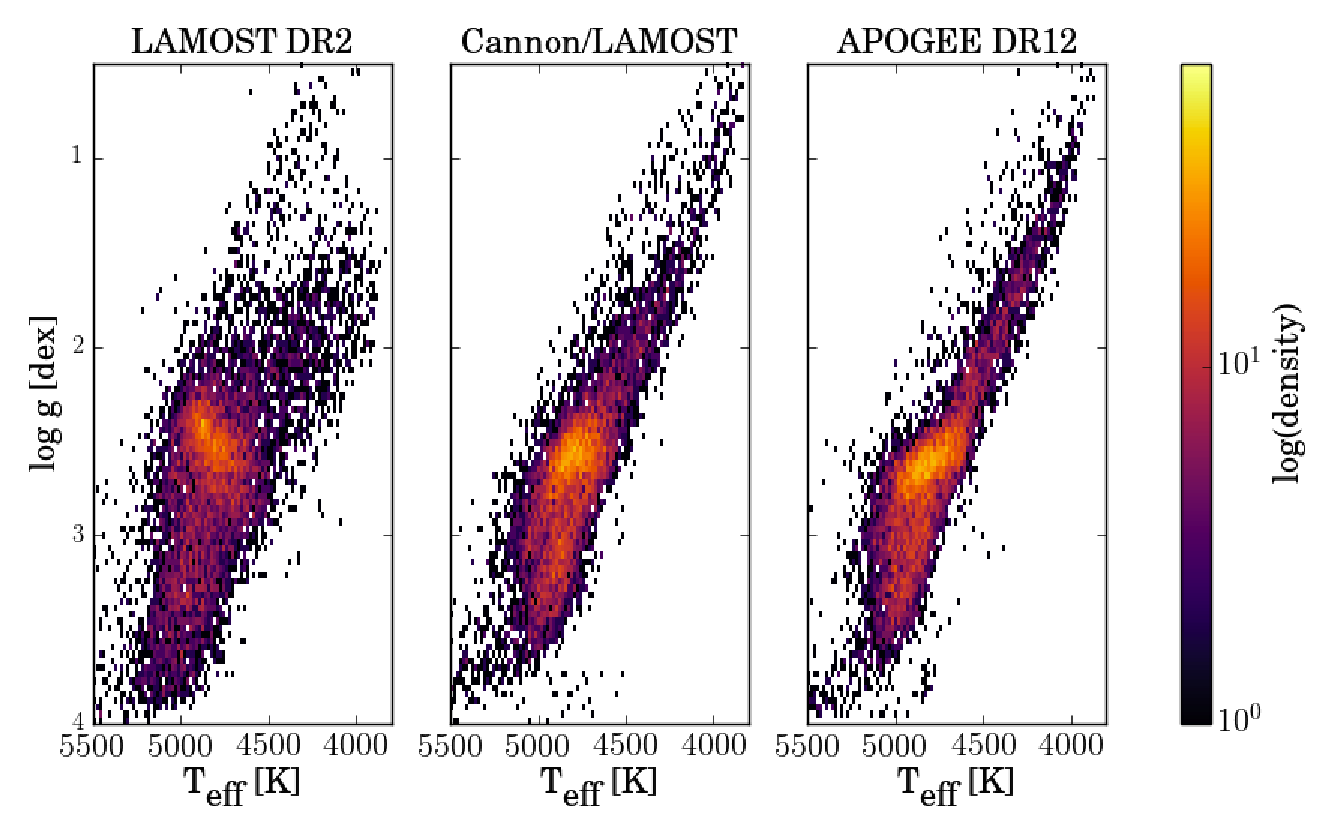
\includegraphics[scale=0.75]{f8.eps}
\caption{Astrophysical verification of the labels derived by \tc\ model for \lamost\ data: the panel show the distribution of all reference objects in the (\teff, \logg) plane, using their \lamost\ DR2 labels (left), Cannon labels from \lamost\ spectra (center), and \apogee~DR12 labels (right). The distribution of Cannon labels is not only much more similar to \aspcap 's labels, but also much more physically plausible, exhibiting a tighter red clump and a more well-defined upper giant branch. }
\label{fig:red-clump}
\end{figure}

We then apply the spectral model to DR2 objects that were \emph{not}
observed by \apogee. \tc\ cannot extrapolate to 
regimes of (\teff, \logg, \feh, \alpham) label space that are completely different
from those represented in the reference set, as shown
in \citet{Ness2015}. Therefore we restrict our test set to \lamost\ 
DR2 objects that are reasonably close to the reference set in label space. 
To do so, we define a ``label-distance" $D$ from the reference objects in label space,
exploiting here that all test objects have (initial) stellar labels estimates from the \lamost\ pipeline. The label-distance of a \lamost\ test object
(in \lamost\ label space; subscript $L$) and a reference object
(in \apogee\ label space; subscript $A$) is

\begin{equation}
D = \frac{1}{K_{\teff}^2} (\teff_{,L}-\teff_{,A})^2 + 
\frac{1}{K_{\logg}^2} (\logg_{L}-\logg_{A})^2 + 
\frac{1}{K_{\feh}^2} (\feh_{L}-\feh_{A})^2 ,
\end{equation}

\noindent where we have normalized by the approximate uncertainty
in each label: $K_{\teff}=100$, $K_{\logg}=0.20$, and $K_{\feh}=0.10$.
We then calculate an object's label-distance from the 
reference set by taking the average of its label-distances to the ten nearest reference objects. 

We use these label-distances to define the regime within which a
\lamost\ DR2 object was deemed a feasible test object. 
The label-distance cut was determined by running the test step of \tc\ on 3,000 random objects in \lamost\ DR2. 
In Figure \ref{fig:ts-dist} we show the label-distance from the Cannon-inferred labels to the original \lamost\ pipeline labels, 
plotted against each object's label-distance from the reference set. Figure \ref{fig:ts-dist} shows a gap along the x-axis, separating the giant branch (close to the reference set) from the main sequence. Figure \ref{fig:ts-dist-dr2} shows 14,000 random stars in the 
(\teff, \logg)-plane (colored points), on top of the entire \lamost\ DR2 sample (see Figure \ref{fig:reference-set-label-space}): a label-distance cut at 2.5 neatly separates the giants (to which the spectral model applies) from the main sequence stars.

\begin{figure}[!p]
\centering
\includegraphics[scale=0.6]{f9.eps}
\caption{Label Distance of LAMOST Objects from Reference Set: Giant branch stars and main sequence stars in \lamost\ DR2 separate out when their distance from reference label space is plotted against the distance from their \lamost\ labels to their Cannon labels, which are determined by running these stars through \tc\ test step.
We use this to inform our choice of test objects: we select those
with a label distance to the reference set of less than 2.5.}
\label{fig:ts-dist}
\end{figure}

\begin{figure}[H]
\centering
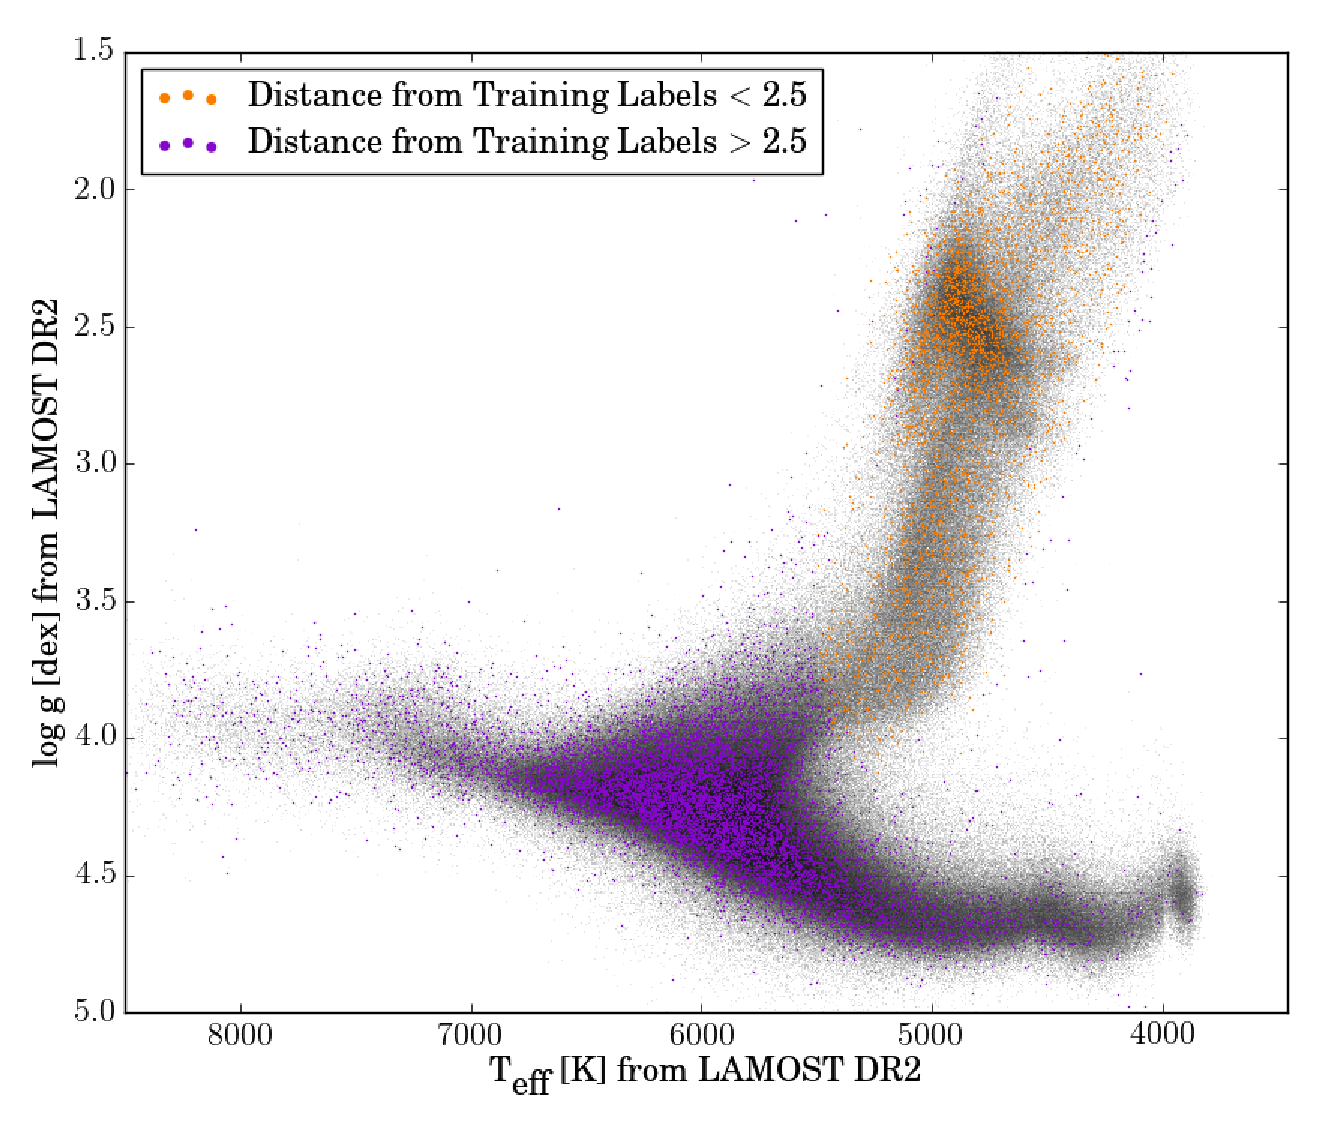
\includegraphics[scale=0.7]{f10.eps}
\caption{Label Distance From Reference Set: (Black) all LAMOST DR2 points in (\teff,\logg) space, with (Color) 14,000 objects overlaid color-coded by their distances from the reference label space. For the test step, we choose objects whose distances are less than 2.5,
which corresponds to the giant branch.}
\label{fig:ts-dist-dr2}
\end{figure}

We define the test set as all \lamost\ DR2 objects with a label-distance from the reference set of $<2.5$.
After using the spectral model to infer new labels,
we excise objects for which the convergence either failed or resulted in a fit with reduced $\chi^2$\,\textgreater\,10 (fewer than 0.1\% of the objects). This leaves \ntestobj\ stars (giants), not including the reference set. 
The newly inferred
labels for these objects, together with the \cannon\ labels for the reference set and their associated formal errors
(from the covariance matrix), are available in a table online and an excerpt is shown in Table \ref{tab:results}. 
This table includes the first-ever \alpham\ values measured from \lamost\ spectra.

In addition to the formal errors from the covariance matrix, there is a contribution to the error on the labels from the discreteness of the reference set. To estimate this, we create \nbssamples\ different spectral models by
bootstrap-sampling from the set of reference objects. For each
set, we run the cross-calibration as described in Figure \ref{fig:cross-validation}. 
A subset of the test set has \nbssamples\ different
label estimates, and we adopt the standard deviation of these measurements as an approximate error bar on these new \lamost\ labels.
With such a large training sample with which to fit the spectral model, the values are negligible: \tefferr\ for \teff, \loggerr\ for \logg, \feherr\ for \feh, and \afeerr\ for \alpham. 
To emphasize, these are not the full errors on the labels, but only the contribution from the incomplete and sometimes sparse coverage of label space by the reference objects. 

\Comment{AYQH}{Add positions to the table.}

\begin{table}[H]
\begin{center}
\caption{Excerpt from the online table of stellar labels (\teff, \logg, \feh, and \alpham) for \nallobj\ stars, 
inferred by \tc\ directly from \lamost\ spectra.
Column 1 is the \lamost\ ID of the object,
Columns 2-5 are the labels from \tc,
Columns 6-9 are the formal errors on those labels from the covariance matrix in the
Cannon model fit,
and the final column is the reduced $\chi^2$.
Note that the reduced $\chi^2$ values are low by a factor of $\sim$\,3  because the random component of the errors
in the \lamost\ spectra is overestimated (see Section \ref{sec:test}).
\label{tab:results}}
{\scriptsize
\begin{tabular}{cccccccccc}
\tableline\tableline
LAMOST ID  & \teff\ & \logg\ & \feh\ & \alpham\ & $\sigma$(\teff) & $\sigma$(\logg) & $\sigma$(\feh) & $\sigma$(\alpham) & Red. \\
& (K) & (dex) & (dex) & (dex) & (K) & (dex) & (dex) & (dex) & $\chi^2$ \\    
\tableline
spec-55859-F5902\_sp01-034.fits & 4899 & 3.15 & -0.597  & 0.207 & 48 & 0.08 & 0.053 & 0.024 & 0.62 \\
spec-55859-F5902\_sp01-136.fits & 5279 &  3.08 & -0.838 & 0.206 & 145 & 0.29 & 0.177 & 0.075 & 0.57 \\
spec-55859-F5902\_sp01-202.fits & 4884 & 3.25 & -0.383 & 0.225 & 36 & 0.06 & 0.040 & 0.016 & 0.82 \\
spec-55859-F5902\_sp01-207.fits & 4882 & 3.43 & -0.252 & 0.186 & 39 & 0.06 & 0.043 & 0.017 & 0.88 \\
\tableline
\end{tabular}}
\end{center}
\end{table}  

\subsection{The \alpham\ Map of the Milky Way from \lamost}

The full astrophysical verification and exploitation of the new set of labels for the \lamost\ DR2 giants is beyond the scope of the paper. 
Here, we give some initial indication of what will be enabled, 
by showing the (\feh,\alpham) plane (Figure \ref{fig:alpha-feh})
and the distribution
of \alpham\ in galactic latitude and longitude
(Figure \ref{fig:am-map})
for all \lamost\ DR2 giants. 
This is by far the largest set of giants with the \alpham\
abundance label. As Fig. \ref{fig:am-map} shows, the combination of the two surveys
overcomes a limitation of many previous analyses of the abundance-dependent Galactic disk structure (see e.g. \cite{RixBovy2013}): most large surveys have either extensive coverage at high Galactic latitudes with sparse sampling in the Galactic plane, or vice versa.
The distribution in the (\feh,\alpham) plane 
looks very plausible, exhibiting the $\alpha$-enhanced and the low-$\alpha$ sequences, and the spatial distribution
beautifully exhibits the low-alpha, chemically late, young
population in the mid-plane and at large radii, and the
alpha-enhanced, rapidly enriched, old population in the thick 
disk (high latitudes) and Galactic center. 

\begin{figure}[H]
\centering
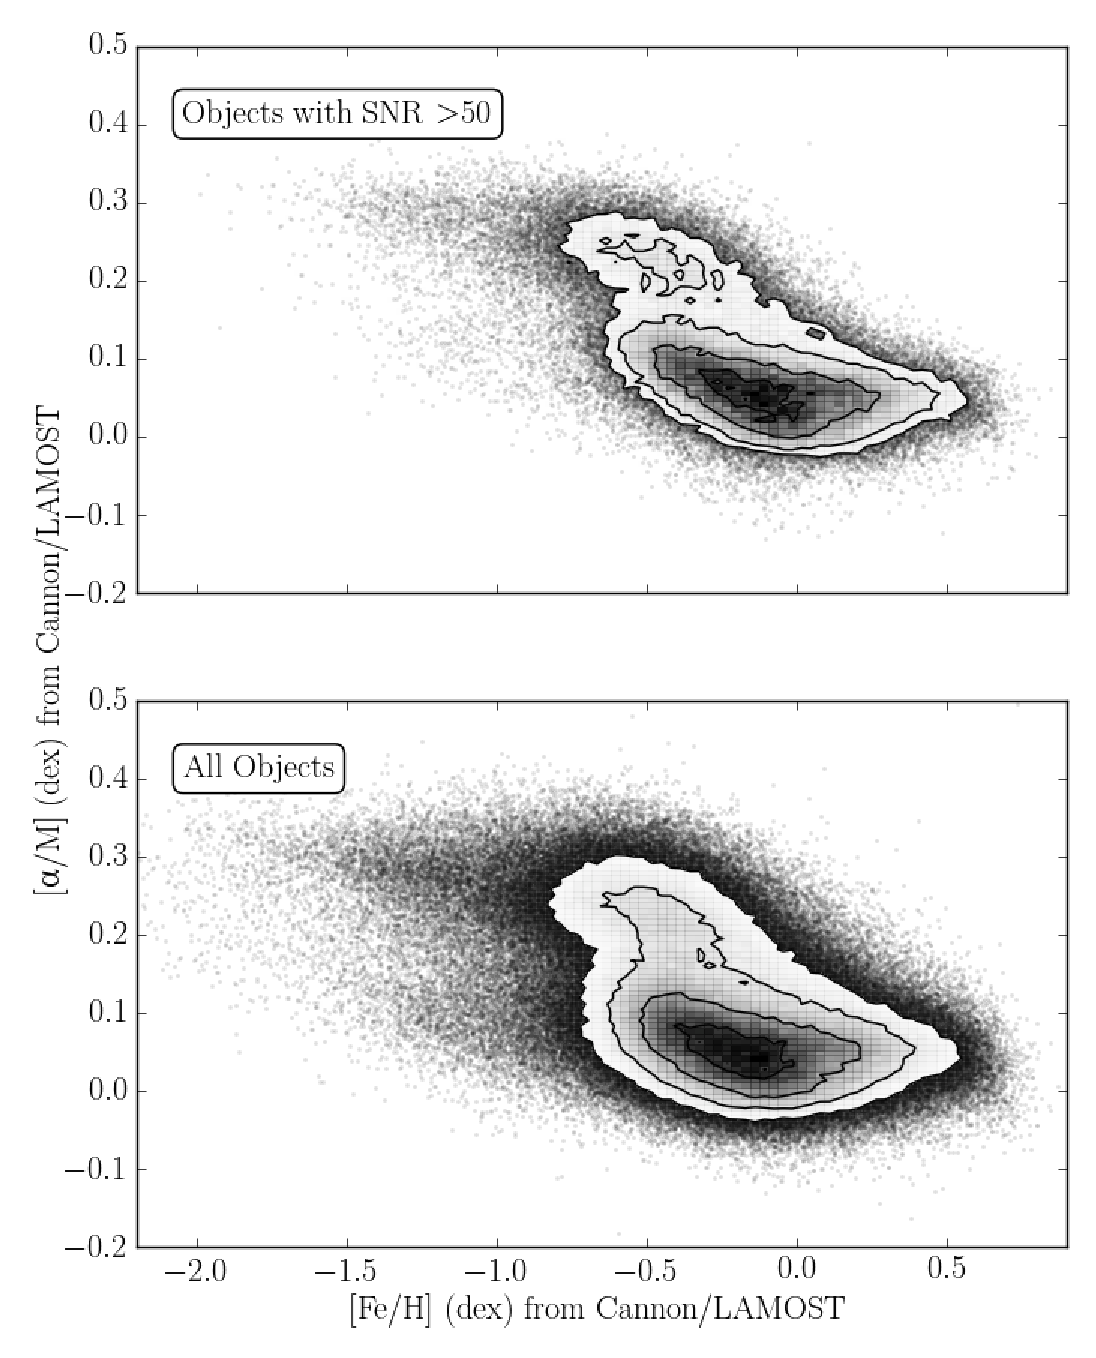
\includegraphics[scale=0.7]{f11.eps}
\caption{The (\alpham, \feh) plane, showing the labels  determined by \tc\ for all \nallobj\ objects.
The raw values are shown as grayscale points and
the contours (made from logarithmic bins) are at 0.5, 1, 1.5, and 2 sigma.
These are the first \alpham\ values measured from \lamost\ spectra,
and by far the largest set of giants with this abundance label. Figure made using code from \citet{DanFM}.
}
\label{fig:alpha-feh}
\end{figure}

\begin{figure}[!p]
\centering
\includegraphics[scale=0.80]{f12.eps}
\caption{The distribution on the sky (in Galactic coordinates) of the
full set of objects with consistently measured 
\alpham : 
the top panel shows
the full \apogee\ sample with
$\approx$\, 100,000 objects,
and the bottom panel shows these values
combined with \nallobj\ \alpham\ inferred by
\tc\ from the \lamost\  spectra. 
The much more extensive area coverage of the \lamost\ data is immediately apparent.
One can clearly see how the low-$\alpha$ stars, presumably a younger population from more slowly enriched gas, is concentrated towards the mid-plane.
The $\alpha$-enhanced stars, mostly a rapidly enriched, old population, are found
in the thick disk and halo (at high latitudes) as well as in the outer Galactic bulge;
the arrow on the right denotes the Galactic center.
This illustrates the promise of survey cross-calibration
for stitching together a more complete stellar population picture of the Galaxy.
}
\label{fig:am-map}
\end{figure}

\section{Discussion}

We have demonstrated that \tc\ can be used to put two 
spectroscopic stellar surveys with very different experimental set-ups (wavelength coverage, resolution) onto the same label (stellar parameter and chemical abundance)
scale by training a spectral model on the set of objects observed in common between
the surveys. We used \lamost\ and \apogee\ as our example, and showed that we can greatly reduce the systematic differences between labels measured using the two individual survey pipelines. 
We can also boost the precision of the label estimates for the data set of less resolution and S/N (\lamost\ in this case).  By training our model to
infer \apogee -scale stellar labels directly from \lamost\ spectra, we
can also transfer new labels from one survey to another for: here we derived \alphafe\ 
from \lamost\ spectra for the first time. 

There are substantial benefits to using \tc\ for survey cross-calibration. As described in \citep{Ness2015}, \tc\ is very fast:
for \ntrobj\ objects, on a regular computer,
the training step took a few minutes and 
the test step for \ntestobj\ test objects 
(i.e. the label determination) took a few hours.
In addition, \tc\ requires no physical models and performs well
at low \snr\ and low resolution: in this case, we were able to measure
labels of comparable precision to \apogee\ (at least, to 
\aspcap's stated precision; see \citet{Ness2015})
from \lamost's substantially lower resolution and lower \snr\ spectra (see Figure \ref{fig:snr-test}).
Finally, because \tc\ fits for a set of model coefficients independently at each wavelength of the spectrum, 
there is a straightforward way to investigate the information content 
of a particular wavelength regime and determine where and how
information about a particular label is encoded (see Figure \ref{fig:leading-coeffs}).

This cross-calibration effort was both enabled and severely limited
by the reference set: the large number of objects with reliable labels (\ntrobj) measured in common between the two surveys enabled us to fit for a spectral model, but the incomplete label coverage 
restricted the applicability of the model to only \nallobj\ out of
several million \lamost\ objects. To take full advantage a data-driven approach like \tc, it is essential
for surveys to measure objects in common that have
high-fidelity labels comprehensively spanning the label space
of interest. 

Clearly, \tc\ holds promise for bringing other overlapping surveys
onto the same label scale (e.g. \rave, \segue, \galah, \gaiaeso). Looking ahead, Gaia will provide a billion low-resolution spectra.
By the time these spectra become available, over a million of these objects will have spectroscopic labels determined by much higher resolution ground-based spectra. This offers a tremendous 
opportunity for transferring high-quality spectral labels to low-resolution Gaia spectra, if not with the present version of \tc\ then with the basic underlying ideas of data-driven spectral modeling.

The code used to produce the results described in this paper was written in
Python and is available online in an open-source repository.\footnote{\url{www.github.com/annayqho/TheCannon}}

\acknowledgements

It is a pleasure to thank 
Jo Bovy (U. Toronto),
Andy Casey (IoA Cambridge),
Morgan Fouesneau (MPIA), 
Evan Kirby (Caltech),
Branimir Sesar (MPIA), and
Yuan-Sen Ting (Harvard)
for valuable discussions and assistance.
AYQH is grateful to the community at the MPIA for 
their support and hospitality during the period in which most of this work was performed. 

AYQH was supported by a Fulbright grant through the German-American Fulbright Commission and a National Science Foundation Graduate Research Fellowship under Grant No. DGE‐1144469. 
MKN and HWR have received funding for this research from the European Research Council under the European Union's Seventh Framework Programme (FP 7) ERC Grant Agreement n. [321035].
DWH was partially supported by the NSF (grant IIS-1124794), NASA (grant NNX08AJ48G), and the Moore-Sloan Data Science Environment at NYU.
CL acknowledges the Strategic Priority Research Program ``The Emergence of Cosmological Structures" of the Chinese Academy of Sciences, Grant No. XDB09000000, the National Key Basic Research Program of China 2014CB845700, and the National Natural Science Foundation of China (NSFC) grants No. 11373032 and 11333003.

Guoshoujing Telescope (the Large Sky Area Multi-Object Fiber Spectroscopic Telescope LAMOST) is a National Major Scientific Project built by the Chinese Academy of Sciences. Funding for the project has been provided by the National Development and Reform Commission. LAMOST is operated and managed by the National Astronomical Observatories, Chinese Academy of Sciences.

Funding for the Sloan Digital Sky Survey IV has been provided by
the Alfred P. Sloan Foundation, the U.S. Department of Energy Office of
Science, and the Participating Institutions. SDSS-IV acknowledges
support and resources from the Center for High-Performance Computing at
the University of Utah. The SDSS web site is www.sdss.org.

SDSS-IV is managed by the Astrophysical Research Consortium for the 
Participating Institutions of the SDSS Collaboration including the 
Brazilian Participation Group, the Carnegie Institution for Science, 
Carnegie Mellon University, the Chilean Participation Group, the French Participation Group, Harvard-Smithsonian Center for Astrophysics, 
Instituto de Astrof\'isica de Canarias, The Johns Hopkins University, 
Kavli Institute for the Physics and Mathematics of the Universe (IPMU) / 
University of Tokyo, Lawrence Berkeley National Laboratory, 
Leibniz Institut f\"ur Astrophysik Potsdam (AIP),  
Max-Planck-Institut f\"ur Astronomie (MPIA Heidelberg), 
Max-Planck-Institut f\"ur Astrophysik (MPA Garching), 
Max-Planck-Institut f\"ur Extraterrestrische Physik (MPE), 
National Astronomical Observatory of China, New Mexico State University, 
New York University, University of Notre Dame, 
Observat\'ario Nacional / MCTI, The Ohio State University, 
Pennsylvania State University, Shanghai Astronomical Observatory, 
United Kingdom Participation Group,
Universidad Nacional Aut\'onoma de M\'exico, University of Arizona, 
University of Colorado Boulder, University of Oxford, University of Portsmouth, 
University of Utah, University of Virginia, University of Washington, University of Wisconsin, 
Vanderbilt University, and Yale University.

{\it Facilities:} \facility{Sloan(APOGEE spectrograph)}, \facility{LAMOST} 

\begin{thebibliography}{24}
\expandafter\ifx\csname natexlab\endcsname\relax\def\natexlab#1{#1}\fi

\bibitem[Alam et al.(2015)]{Alam2015} Alam, S., Albareti, F.~D., 
Allende Prieto, C., et al.\ 2015, \apjs, 219, 12 

\bibitem[Bovy et al.(2012)]{Bovy2012} Bovy, J., Rix, H.-W., Hogg, D.~W., et al.\ 2012, \apj, 755, 115

\bibitem[Chen et al.(2015)]{Chen2015} Chen, Y.~Q., Zhao, G., 
Liu, C., et al.\ 2015, arXiv:1506.00771 

\bibitem[De Silva et al.(2015)]{DeSilva2015} De Silva, G.~M., 
Freeman, K.~C., Bland-Hawthorn, J., et al.\ 2015, \mnras, 449, 2604 

\bibitem[Eisenstein et al.(2011)]{Eisenstein2011} Eisenstein, D.~J., 
Weinberg, D.~H., Agol, E., et al.\ 2011, \aj, 142, 72 

\bibitem[Dan Foreman-Mackey et al.(2014)]{DanFM}
Foreman-Mackey, D., et al. triangle.py v0.1.1. Zenodo. 10.5281/zenodo.11020

\bibitem[Friedman et al.(2011)]{Friedman2011} Friedman, S.~D., York, 
D.~G., McCall, B.~J., et al.\ 2011, \apj, 727, 33 

\bibitem[Garc{\'{\i}}a P{\'e}rez et al.(2015)]{GarciaPerez2015} 
Garc{\'{\i}}a P{\'e}rez, A.~E., Allende Prieto, C., Holtzman, J.~A., et 
al.\ 2015, arXiv:1510.07635 

\bibitem[{{Gilmore} {et~al.}(2012){Gilmore}, {Randich}, {Asplund}, {Binney},
  {Bonifacio}, {Drew}, {Feltzing}, {Ferguson}, {Jeffries}, {Micela},
  {Negueruela}, {Prusti}, {Rix}, {Vallenari}, {Alfaro}, {Allende-Prieto},
  {Babusiaux}, {Bensby}, {Blomme}, {Bragaglia}, {Flaccomio}, {Fran{\c c}ois},
  {Irwin}, {Koposov}, {Korn}, {Lanzafame}, {Pancino}, {Paunzen},
  {Recio-Blanco}, {Sacco}, {Smiljanic}, {Van Eck}, \& {Walton}}]{Gilmore2012}
{Gilmore}, G., {Randich}, S., {Asplund}, M., {Binney}, J., {Bonifacio}, P.,
  {Drew}, J., {Feltzing}, S., {Ferguson}, A., {Jeffries}, R., {Micela}, G.,
  {Negueruela}, I., {Prusti}, T., {Rix}, H.-W., {Vallenari}, A., {Alfaro}, E.,
  {Allende-Prieto}, C., {Babusiaux}, C., {Bensby}, T., {Blomme}, R.,
  {Bragaglia}, A., {Flaccomio}, E., {Fran{\c c}ois}, P., {Irwin}, M.,
  {Koposov}, S., {Korn}, A., {Lanzafame}, A., {Pancino}, E., {Paunzen}, E.,
  {Recio-Blanco}, A., {Sacco}, G., {Smiljanic}, R., {Van Eck}, S., \& {Walton},
  N. 2012, The Messenger, 147, 25

\bibitem[Gunn et al.(2006)]{Gunn2006} Gunn, J.~E., Siegmund, 
W.~A., Mannery, E.~J., et al.\ 2006, \aj, 131, 2332 

\bibitem[Herbig(1993)]{Herbig1993} Herbig, G.~H.\ 1993, \apj, 407, 142 

\bibitem[Herbig(1995)]{Herbig1995} Herbig, G.~H.\ 1995, \araa, 33, 19 

\bibitem[Hobbs et al.(2008)]{Hobbs2008} Hobbs, L.~M., York, 
D.~G., Snow, T.~P., et al.\ 2008, \apj, 680, 1256 

\bibitem[Holtzman et al.(2015)]{Holtzman2015} Holtzman, J.~A., 
Shetrone, M., Johnson, J.~A., et al.\ 2015, arXiv:1501.04110 

\bibitem[Kordopatis et al.(2013)]{Kordopatis2013} Kordopatis, G., 
Gilmore, G., Steinmetz, M., et al.\ 2013, \aj, 146, 134 

\bibitem[Liu et al.(2014)]{Liu2014} Liu, C., Deng, L.-C., 
Carlin, J.~L., et al.\ 2014, \apj, 790, 110 

\bibitem[Liu et al.(2015)]{Liu2015} Liu, C., Fang, M., Wu, Y., 
et al.\ 2015, \apj, 807, 4 

\bibitem[Luo A.L., Bai Z.R. et al.(2015)]{Luo2015} Luo, A.L., Bai, Z.~R., et al.\ 2015, RAA, in press

\bibitem[{{Majewski et al.}(2015)}]{Majewski2015} Majewski, S. R., Schiavon, R. P., Allende Prieto, C., et al.\ 2015, in preparation

\bibitem[McCall et al.(2010)]{McCall2010} McCall, B.~J., Drosback, 
M.~M., Thorburn, J.~A., et al.\ 2010, \apj, 708, 1628 

\bibitem[M{\'e}sz{\'a}ros et al.(2013)]{Meszaros2013} 
M{\'e}sz{\'a}ros, S., Holtzman, J., Garc{\'{\i}}a P{\'e}rez, A.~E., et al.\ 
2013, \aj, 146, 133 

\bibitem[Ness et al.(2015)]{Ness2015} Ness, M., Hogg, D.~W., 
Rix, H.-W., Ho, A.~Y.~Q., \& Zasowski, G.\ 2015, \apj, 808, 16 

\bibitem[Ness et al.(2016)]{NessAges} Ness, M., Hogg, D.~W., 
Rix, H., et al.\ 2016, arXiv:1511.08204 

\bibitem[Rix 
\& Bovy(2013)]{RixBovy2013} Rix, H.-W., \& Bovy, J.\ 2013, \aapr, 21, 61 

\bibitem[Sarre(2006)]{Sarre2006} Sarre, P.~J.\ 2006, Journal of 
Molecular Spectroscopy, 238, 1 

\bibitem[Smiljanic et 
al.(2014)]{Smiljanic2014} Smiljanic, R., Korn, A.~J., Bergemann, M., et al.\ 2014, \aap, 570, A122 

\bibitem[Wan et al.(2015)]{Wan2015} Wan, J.-C., Liu, C., Deng, 
L.-C., et al.\ 2015, Research in Astronomy and Astrophysics, 15, 1166 

\bibitem[Wilson et al.(2010)]{Wilson2010} Wilson, J.~C., Hearty, 
F., Skrutskie, M.~F., et al.\ 2010, \procspie, 7735, 77351C 

\bibitem[Wu et al.(2011)]{Wu2011} Wu, Y., Luo, A.-L., Li, 
H.-N., et al.\ 2011, Research in Astronomy and Astrophysics, 11, 924 

\bibitem[Yanny et al.(2009)]{Yanny2009} Yanny, B., Rockosi, C., 
Newberg, H.~J., et al.\ 2009, \aj, 137, 4377-4399 

\bibitem[Yuan 
\& Liu(2012)]{Yuan2012} Yuan, H.~B., \& Liu, X.~W.\ 2012, \mnras, 425, 1763 

\bibitem[Zasowski et al.(2015)]{Zasowski2015} Zasowski, G., 
M{\'e}nard, B., Bizyaev, D., et al.\ 2015, \apj, 798, 35 

\bibitem[Zhao et al.(2012)]{Zhao2012} Zhao, G., Zhao, Y.-H., 
Chu, Y.-Q., Jing, Y.-P., 
\& Deng, L.-C.\ 2012, Research in Astronomy and Astrophysics, 12, 723 

\end{thebibliography}

\end{document}
